\section{Policy Background}
\label{sec:policy}

The EU~ETS, established by Directive 2003/87/EC \citep{directive2003}, operates as a cap-and-trade system covering CO$_2$ emissions from power generation and energy-intensive manufacturing across the European Economic Area. Its four phases differ in allocation rules that directly shape the proposed treatment variable (Figure~\ref{fig:timeline}).

\paragraph{Phase~I (2005--2007).}
National allocation plans (NAPs) distributed allowances for free on the basis of historical emissions. Over-allocation was widespread, the EUA spot price collapsed to near zero by mid-2007, and Phase~I allowances could not be banked \citep{ellerman2016}. The effective carbon cost was therefore negligible, a feature the proposed treatment variable captures mechanically.

\paragraph{Phase~II (2008--2012).}
The cap tightened, NAPs underwent stricter Commission review, and banking into Phase~III was permitted. The EUA price reached approximately EUR~25 in mid-2008 before falling to EUR~8 during the financial crisis. Free allocation remained dominant, with auctioning below 4 per cent of allowances \citep{ellerman2016}.

\paragraph{Phase~III (2013--2020).}
EU-wide harmonised rules replaced NAPs. Auctioning became the default for the power sector; manufacturing sectors on the carbon-leakage list received free allocation at product-specific benchmarks set at the 10 per cent most efficient installations. This benchmark-based system introduced cross-sectoral variation in $a_{st}$ independent of installation behaviour, providing the sector-year variation on which the proposed treatment relies. The EUA price remained below EUR~10 for most of 2013 to 2017, partly due to a cumulative surplus of approximately 2 billion allowances.

\paragraph{Market Stability Reserve and price acceleration.}
The MSR, established by Decision (EU) 2015/1814 \citep{msr2015}, began operating in January 2019 and withdrew surplus allowances from circulation. The EUA price rose from EUR~8 in early 2018 to EUR~25 by end-2019 and exceeded EUR~50 in 2021, generating the strongest effective treatment in the proposed sample.

\paragraph{Phase~IV (from 2021) and CBAM.}
The revised Directive tightened the cap reduction factor and reduced free allocation. The proposed sample includes only 2021 from Phase~IV. The Carbon Border Adjustment Mechanism (CBAM), proposed in July 2021 and adopted as Regulation (EU) 2023/956 \citep{cbam2023}, imposes a carbon cost on imports of cement, iron and steel, aluminium, fertilisers, electricity, and hydrogen. Its transitional phase began in October 2023; the definitive regime phases in from 2026 as free allocation is phased out. CBAM's product scope coincides with North African emission-intensive exports to the EU, making this corridor a direct test of the conditions the mechanism addresses. The July 2021 proposal could induce anticipation effects in the final sample year, but anticipation of a border charge deters leakage and would bias the estimated coefficient toward zero. The event-study specification would detect any discontinuous 2021 shift.

\begin{figure}[htbp]
\centering
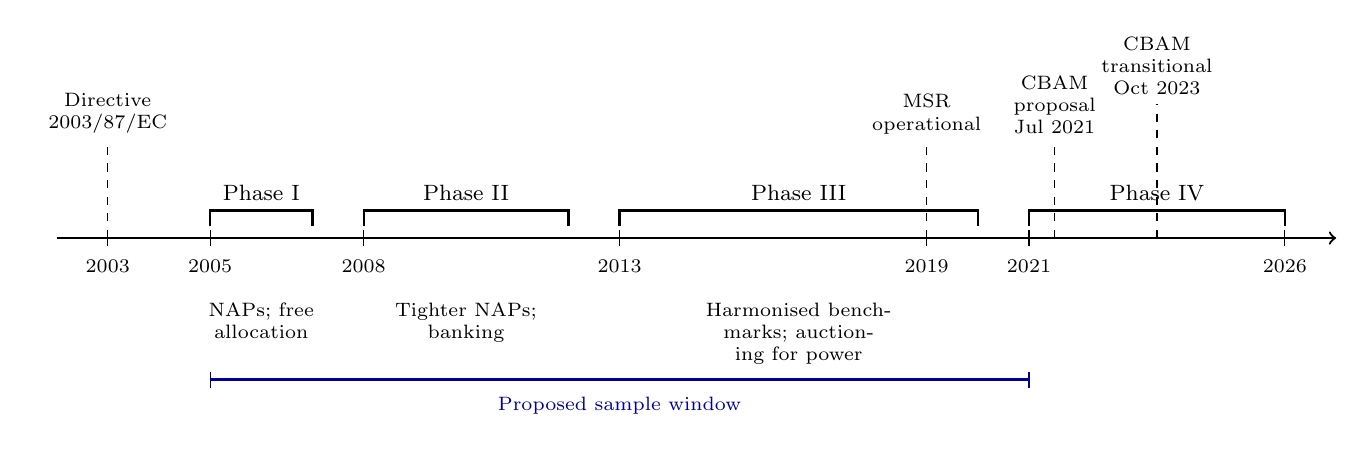
\begin{tikzpicture}[x=0.65cm, y=1cm]

  \draw[thick, ->] (2,0) -- (27,0);

  \draw[thick] (5,0.15) -- (5,0.35) -- (7,0.35) -- (7,0.15);
  \node[above] at (6,0.35) {\footnotesize Phase~I};

  \draw[thick] (8,0.15) -- (8,0.35) -- (12,0.35) -- (12,0.15);
  \node[above] at (10,0.35) {\footnotesize Phase~II};

  \draw[thick] (13,0.15) -- (13,0.35) -- (20,0.35) -- (20,0.15);
  \node[above] at (16.5,0.35) {\footnotesize Phase~III};

  \draw[thick] (21,0.15) -- (21,0.35) -- (26,0.35) -- (26,0.15);
  \node[above] at (23.5,0.35) {\footnotesize Phase~IV};

  \foreach \y/\l in {3/2003, 5/2005, 8/2008, 13/2013, 19/2019, 21/2021, 26/2026} {
    \draw (\y,-0.1) -- (\y,0.1);
    \node[below, font=\scriptsize] at (\y,-0.15) {\l};
  }

  \node[below, font=\scriptsize, text width=1.8cm, align=center] at (6,-0.7) {NAPs; free allocation};
  \node[below, font=\scriptsize, text width=2.2cm, align=center] at (10,-0.7) {Tighter NAPs; banking};
  \node[below, font=\scriptsize, text width=3cm, align=center] at (16.5,-0.7) {Harmonised benchmarks; auctioning for power};

  \draw[dashed] (3,0) -- (3,1.2);
  \node[above, font=\scriptsize, text width=1.8cm, align=center] at (3,1.2) {Directive 2003/87/EC};

  \draw[dashed] (19,0) -- (19,1.2);
  \node[above, font=\scriptsize, text width=1.5cm, align=center] at (19,1.2) {MSR operational};

  \draw[dashed] (21.5,0) -- (21.5,1.2);
  \node[above, font=\scriptsize, text width=1.5cm, align=center] at (21.5,1.2) {CBAM proposal Jul 2021};

  \draw[dashed] (23.5,0) -- (23.5,1.7);
  \node[above, font=\scriptsize, text width=1.8cm, align=center] at (23.5,1.7) {CBAM transitional Oct 2023};

  \draw[very thick, blue!60!black] (5,-1.8) -- (21,-1.8);
  \draw[blue!60!black] (5,-1.9) -- (5,-1.7);
  \draw[blue!60!black] (21,-1.9) -- (21,-1.7);
  \node[below, font=\scriptsize, blue!60!black] at (13,-1.9) {Proposed sample window};

\end{tikzpicture}
\caption{EU~ETS institutional timeline. The four trading phases, key regulatory events, and the proposed sample window (2005--2021). Institutional facts only; no price data plotted.}
\label{fig:timeline}
\end{figure}
